\documentclass[12pt]{article}
\usepackage[margin=1in]{geometry} % Create 1 inch margins
\usepackage{natbib} % Citation package 
\usepackage{indentfirst} % Indent the first paragraph of the 1st paragraph of each new section. 
\usepackage{setspace} % Package to set my line spacing
\usepackage[bottom]{footmisc}
\doublespacing % declare double space
\interfootnotelinepenalty=999999999
\usepackage{sectsty}
\sectionfont{\normalfont\fontfamily{ptm}\fontsize{12}{12}\bfseries}
\subsectionfont{\normalfont\fontfamily{ptm}\fontsize{12}{12}\itshape}
\usepackage{times} % Text font as TNR
\usepackage{graphicx} % Include images 
%\usepackage[none]{hyphenat} % Stops breaking up words at the right side of the page. 
\usepackage{comment} % Pakeage to let me comment out large secitons at a time.
\usepackage{xurl} % Fix urls on the page
\usepackage{graphicx} % Include Graphics
\usepackage{array}
\usepackage{caption}
\usepackage{subcaption}
\usepackage{hyperref} % Hyperlink to figures and bibliography
\usepackage{fancyhdr} % All of this is to put the page number at the bottom right
\pagestyle{fancy}
\fancyhead{}
\fancyfoot{}
\fancyfoot[R]{\thepage}
\renewcommand{\headrulewidth}{0pt} % This says to not put the line at the top of the apge that makes it "fancy".
\setlength{\parindent}{1cm}
\renewcommand{\thesection}{\Roman{section}}
\renewcommand{\thesubsection}{\thesection.\Roman{subsection}}
\usepackage{soul} % Fix wrapping of underlined text
\usepackage[font=small]{caption} %Change the size of the "Figre XX" caption part. 
\usepackage{xcolor}
\usepackage{import}
\usepackage{tikz,pgfplots}
\usepackage{tkz-graph}
\usetikzlibrary{arrows.meta}
\usetikzlibrary{positioning}
\usepackage{titling}
\usepackage{pdflscape}
\usepackage{rotating}
\usepackage{appendix}

\title{UN-Interested Suppliers \\
\large Effects of Peacekeeping Mandates on Contributions \\
\large \textbf{Oneline Appendix}}
\author{Robert Wood \\
University of Kentucky}
\date{\today}

\begin{document}

\begin{titlingpage}
\maketitle
\end{titlingpage}

\appendix 

\renewcommand{\thesection}{Appendix \Alph{section}}
\setcounter{section}{0}

\renewcommand{\thetable}{\Alph{section}\arabic{table}}
\setcounter{table}{0}

\renewcommand{\thefigure}{\Alph{section}\arabic{figure}}
\setcounter{figure}{0}

\begin{landscape}
\begin{centering}
\section{}
\end{centering}
\begin{table}[htbp]\centering
\fontsize{7}{7}\selectfont
\def\sym#1{\ifmmode^{#1}\else\(^{#1}\)\fi}
\caption{Model Robustness Checks}
\begin{tabular}{l*{14}{c}}
\hline\hline
&\multicolumn{2}{c}{\ul{All Battle Deaths}}&\multicolumn{2}{c}{\ul{Observer Missions}}&\multicolumn{2}{c}{\ul{30 Contributors}}&\multicolumn{2}{c}{\ul{Same Continent, MP}}&\multicolumn{2}{c}{\ul{Ever Sent}}&\multicolumn{4}{c}{\ul{Zero-Inflated Negative Binomial}}\\
[0.2em]
&\multicolumn{1}{c}{Model 6}&\multicolumn{1}{c}{Model 7}&\multicolumn{1}{c}{Model 8}&\multicolumn{1}{c}{Model 9}&\multicolumn{1}{c}{Model 10}&\multicolumn{1}{c}{Model 11}&\multicolumn{1}{c}{Model 12}&\multicolumn{1}{c}{Model 13}&\multicolumn{1}{c}{Model 14}&\multicolumn{1}{c}{Model 15}&\multicolumn{1}{c}{Model 16}&\multicolumn{1}{c}{Inflate}&\multicolumn{1}{c}{Model 17}&\multicolumn{1}{c}{Inflate}\\
[0.2em]
\hline
Risk Ratio$_{t-1}$ &-2.174\sym{**}&-2.145\sym{**}&-1.832\sym{**}&-1.667\sym{**}&-2.240\sym{**}&-1.982\sym{**}&-3.813\sym{**}&-3.603\sym{**}&-2.879\sym{**}&-2.555\sym{**}&-2.648\sym{**}&&-2.271\sym{**}\\
&(0.431)&(0.431)&(0.450)&(0.477)&(0.499)&(0.521)&(0.760)&(0.839)&(0.498)&(0.529)&(0.516)&&(0.546)\\
[0.5em]
Battle Deaths$_{t-1}$ (Hundreds) &0.000&0.040\sym{*}&0.118&1.535\sym{**}&0.099&2.734\sym{**}&0.637\sym{**}&2.283\sym{\dagger}&0.279\sym{\dagger}&3.302\sym{**}&0.288\sym{*}&&3.652\sym{**}\\
&(0.001)&(0.017)&(0.110)&(0.503)&(0.109)&(0.640)&(0.207)&(1.255)&(0.145)&(0.777)&(0.142)&&(0.738)\\
[0.5em]
Risk Ratio$_{t-1}$ X Battle Deaths$_{t-1}$ &&-0.040\sym{*}&&-1.885\sym{**}&&-3.516\sym{**}&&-2.202&&-3.982\sym{**}&&&-4.437\sym{**}\\
&&(0.017)&&(0.661)&&(0.845)&&(1.666)&&(0.962)&&&(0.924)\\
[0.5em]
Number of Contributors$_{t-1}$ (Tens) &-0.091\sym{**}&-0.088\sym{**}&0.007&0.007&-0.083\sym{*}&-0.088\sym{*}&-0.011&-0.005&-0.037&-0.036&-0.149\sym{*}&-0.294\sym{**}&-0.155\sym{*}&-0.301\\
&(0.034)&(0.034)&(0.036)&(0.037)&(0.036)&(0.038)&(0.080)&(0.079)&(0.044)&(0.045)&(0.061)&(0.078)&(0.063)&(0.079)\\
[0.5em]
Re-hatted$_{t-1}$ &-0.131&-0.122&0.098&0.100&-0.094&-0.093&0.946\sym{**}&0.950\sym{**}&0.099&0.104&0.088&&0.101\\
&(0.144)&(0.144)&(0.163)&(0.163)&(0.163)&(0.162)&(0.258)&(0.258)&(0.169)&(0.170)&(0.195)&&(0.194)\\
[0.5em]
Previous UN Mission$_{t-1}$ &0.553\sym{**}&0.539\sym{**}&0.545\sym{**}&0.546\sym{**}&0.701\sym{**}&0.694\sym{**}&0.889\sym{**}&0.862\sym{**}&0.780\sym{**}&0.766\sym{**}&0.862\sym{**}&&0.862\sym{**}\\
&(0.129)&(0.131)&(0.134)&(0.135)&(0.139)&(0.141)&(0.197)&(0.206)&(0.159)&(0.160)&(0.140)&&(0.143)\\
[0.5em]
Contributor GDP per Capita$_{t-1}$ (Ten Thousands)&-0.125\sym{*}&-0.124\sym{*}&-0.150\sym{**}&-0.149\sym{**}&-0.063&-0.061&0.062&0.058&-0.088&-0.085&0.028&0.181&0.030&0.180\\
&(0.052)&(0.052)&(0.055)&(0.055)&(0.057)&(0.056)&(0.081)&(0.081)&(0.056)&(0.056)&(0.110)&(0.267)&0.105)&(0.253)\\
[0.5em]
Contributor Democracy$_{t-1}$ &2.181\sym{**}&2.188\sym{**}&2.572\sym{**}&2.553\sym{**}&1.567\sym{**}&1.533\sym{**}&2.564\sym{**}&2.537\sym{**}&2.293\sym{**}&2.264\sym{**}&0.837&-5.007\sym{\dagger}&0.785&-4.999\sym{*}\\
&(0.496)&(0.496)&(0.512)&(0.512)&(0.454)&(0.452)&(0.524)&(0.520)&(0.469)&(0.467)&(0.556)&(2.613)&(0.530)&(2.437)\\
[0.5em]
Total Contributed Troops$_{t-1}$ (Hundreds) &0.025\sym{**}&0.025\sym{**}&0.030\sym{**}&0.030\sym{**}&0.038\sym{**}&0.037\sym{**}&0.056\sym{**}&0.055\sym{**}&0.059\sym{**}&0.058\sym{**}&0.053\sym{**}&&0.052\sym{**}\\
&(0.008)&(0.008)&(0.010)&(0.010)&(0.011)&(0.010)&(0.020)&(0.019)&(0.015)&(0.015)&(0.016)&&(0.016)\\
[0.5em]
Proportion of Contributor Troops$_{t-1}$ &1.288\sym{*}&1.286\sym{*}&0.981&0.979&1.200&1.200&0.533&0.511&1.954&1.895&2.800&&2.709\\
&(0.560)&(0.561)&(0.610)&(0.610)&(0.906)&(0.905)&(0.575)&(0.570)&(2.972)&(2.861)&(3.695)&&(3.500)\\
[0.5em]
Same Continent$_{t-1}$ &0.002&-0.004&-0.030&-0.028&0.193&0.195&&&0.472\sym{*}&0.467\sym{*}&0.245&-0.813&0.229&-0.821\\
&(0.168)&(0.167)&(0.172)&(0.169)&(0.173)&(0.169)&&&(0.228)&(0.225)&(0.262)&(0.718)&(0.256)&(0.701)\\
[0.5em]
Trade$_{t-1}$ (Billions) &0.178\sym{*}&0.177\sym{*}&0.168\sym{\dagger}&0.163\sym{\dagger}&0.089&0.084&-0.007&-0.009&-0.012&-0.015&-0.035&-21.523\sym{*}&-0.039&-21.387\sym{*}\\
&(0.070)&(0.070)&(0.092)&(0.089)&(0.072)&(0.068)&(0.041)&(0.042)&(0.045)&(0.045)&(0.039)&(9.140)&(0.038)&(8.929)\\
[0.5em]
Joint IOs$_{t-1}$ &0.020\sym{**}&0.020\sym{**}&0.033\sym{**}&0.032\sym{**}&0.028\sym{**}&0.027\sym{**}&0.010&0.009&0.020\sym{*}&0.019\sym{*}&0.012&-0.055\sym{**}&0.011&-0.056\sym{**}\\
&(0.007)&(0.007)&(0.008)&(0.008)&(0.007)&(0.007)&(0.013)&(0.013)&(0.009)&(0.008)&(0.012)&(0.015)&(0.012)&(0.015)\\
[0.5em]
Troops$_{t-1}$ &0.504\sym{**}&0.506\sym{**}&0.587\sym{**}&0.587\sym{**}&0.752\sym{**}&0.751\sym{**}&1.351\sym{**}&1.360\sym{**}&1.690\sym{**}&1.692\sym{**}&1.459\sym{**}&&1.454\sym{**}\\
&(0.083)&(0.084)&(0.097)&(0.097)&(0.130)&(0.129)&(0.192)&(0.193)&(0.273)&(0.274)&(0.253)&&(0.251)\\
[0.5em]
Constant &2.087\sym{**}&2.045\sym{**}&0.676&0.573&1.154\sym{\dagger}&1.010\sym{\dagger}&0.493&0.356&-0.534&-0.738&0.830&4.287\sym{**}&0.628&4.326\sym{**}\\
&(0.565)&(0.573)&(0.616)&(0.616)&(0.595)&(0.600)&(0.665)&(0.673)&(0.629)&(0.637)&(0.846)&(0.716)&(0.844)&(0.717)\\
\hline
lnalpha &1.865\sym{**}&1.864\sym{**}&2.038\sym{**}&2.037\sym{**}&2.425\sym{**}&2.422\sym{**}&3.334\sym{**}&3.332\sym{**}&3.533\sym{**}&3.529\sym{**}&\multicolumn{2}{c}{3.355\sym{**}}&\multicolumn{2}{c}{3.346\sym{**}}\\
&(0.088)&(0.088)&(0.095)&(0.095)&(0.077)&(0.078)&(0.126)&(0.126)&(0.087)&(0.087)&\multicolumn{2}{c}{(0.186)}&\multicolumn{2}{c}{(0.181)}\\
\hline
Observations&79097&79097&86253&86253&112492&112492&133629&133629&363427&363427&\multicolumn{2}{c}{442899}&\multicolumn{2}{c}{442899}\\
\hline\hline
\multicolumn{11}{l}{\fontsize{7}{7}\selectfont State clustered standard errors in parentheses}\\
\multicolumn{11}{l}{\fontsize{7}{7}\selectfont Dependent variable is troop counts.}\\
\multicolumn{11}{l}{\fontsize{7}{7}\selectfont \sym{\dagger}\(p<0.10\), \sym{*}\(p<0.05\), \sym{**}\(p<0.01\). Two-tailed test.}\\
\end{tabular}
\end{table}
\vspace{-10mm}

\end{landscape}


\begin{figure}[t!]
\center{\includegraphics[height=4in]{gg_M13_sim.jpg}}
\caption{\small Marginal effect of risk ratio on contributions conditional on battle deaths with 95\% confidence intervals from Model 13.}
\label{fig:Figure 6}
\end{figure}

\clearpage

\begin{centering}
\section{}
\setcounter{table}{0}
\end{centering}

\vspace{-3em}

\begin{singlespace}
\begin{center}
\begin{table}[htbp!]\centering
\fontsize{12}{12}\selectfont
{\def\sym#1{\ifmmode^{#1}\else\(^{#1}\)\fi}
\caption{Missions Included in Sample \label{Table 4}}
\begin{tabular}{l*{4}{c}}
\hline\hline
MINURCA    &   MINURCAT  &   UNISFA   & UNMEE     \\
[1em]
MINURSO    &   MINUSCA   &   UNMIH    & UNMIL     \\
[1em]
MINUSMA    &   MINUSTAH  &   UNMIS    & UNMISET   \\
[1em]
MONUC      &   MONUSCO   &   UNMISS   & UNOCI     \\
[1em]
ONUB       &   ONUCA     &   UNOSOM   & UNOSOM II \\
[1em]
ONUMOZ     &   UNAMIC    &   UNPREDEP & UNPROFOR  \\
[1em]
UNAMID     &   UNAMIR    &   UNSMIH   & UNTAC     \\
[1em]
UNAMSIL    &   UNCRO     &   UNTAES   & UNTAET    \\
[1em]
UNDOF      &   UNFICYP   &   UNTMIH   & UNTSO     \\
[1em]
UNIFIL     &   UNIKOM    &            &           \\
\hline\hline
\end{tabular}
}
\vspace{-1em}
\end{table}

\end{center}
\end{singlespace}

\newpage

\begin{centering}
\section{}
\setcounter{table}{0}
\end{centering}

\begin{table}[htbp]\centering
\fontsize{9.5}{9.5}\selectfont
\def\sym#1{\ifmmode^{#1}\else\(^{#1}\)\fi}
\caption{Meta Analysis of 10 Random Samples \label{Table 9}}
\begin{tabular}{l*{4}{c}}
\hline\hline
        &\multicolumn{1}{c}{15 Non-Contributors}     &\multicolumn{1}{c}{30 Non-Contributors}  & \multicolumn{1}{c}{15 w/ Interaction}  & \multicolumn{1}{c}{30 w/ Interaction}      \\
\hline
Risk Ratio$_{t-1}$ & -1.989           &      -2.414        &    -1.736           &    -2.166   \\
 &                 [-2.283, -1.695]   &   [-2.709, -2.119] &  [-2.041, -1.431]   &  [-2.475, -1.858]  \\
[0.25em]
Battle Deaths$_{t-1}$ (Hundreds)  &         &              &          2.567       &  2.642  \\
        &                           &                      &    [2.188, 2.946]    & [2.234, 3.051] \\
[0.25em]
Risk Ratio$_{t-1}$ X Battle Deaths$_{t-1}$  &   &    &     -3.431          &        -3.361 \\
                    &               &                &   [-3.939, -2.924]  &   [-3.903, -2.819] \\ 
\hline\hline
\multicolumn{5}{l}{\fontsize{8}{8}\selectfont 95\% Confidence intervals presented in brackets.}\\
\multicolumn{5}{l}{\fontsize{8}{8}\selectfont Dependent variable is troop counts. Common effect model with inverse-variance.}\\
\multicolumn{5}{l}{\fontsize{8}{8}\selectfont Read as overall effect size across all 10 samples.}
\end{tabular}
\vspace{-3em}
\end{table}

\clearpage

\begin{centering}
\section{}
\setcounter{table}{0}
\end{centering}


\begin{doublespace}

To demonstrate that battle deaths does not predict mandate risk, I estimate a fractional logistic regression since the dependent variable is bound between 0 and 1. The unit of analysis for this model is the mission-month as it best captures the variation in the level of mandate risk. I include controls related to conflict conditions and the host state to limit potential confounders and cluster the standard errors on the mission. The results can be found in Table \ref{Fraq}. A few control variables are statistically significant such as conflict termination, conflict duration, host GDP per capita, and host democracy, but battle deaths does not approach statistical significance in neither the naive model or the full model. This suggests that the two independent variables of interest are not mutually reinforcing allowing for valid inference between mandate risk and battle deaths on troop contributions.

\end{doublespace}

\vspace{-0.5em}

\begin{table}[htbp]\centering
\footnotesize
\def\sym#1{\ifmmode^{#1}\else\(^{#1}\)\fi}
\caption{Predicting Mandate Risk with Conflict Dynamics\label{Fraq}}
\begin{tabular}{l*{2}{c}}
\hline\hline
                    &\multicolumn{1}{c}{Model 18}        &\multicolumn{1}{c}{Model 19}        \\
\hline
Battle Deaths$_{t-1}$ (Hundreds)&      -0.143        &      -0.066        \\
                    &     (0.275)        &     (0.204)        \\
[0.5em]
Number of Contributors$_{t-1}$&                    &      -0.137        \\
                    &                    &     (0.093)        \\
[0.5em]
Previous UN Mission$_{t-1}$ &                    &       0.389        \\
                    &                    &     (0.370)        \\
[0.5em]
Re-hatted$_{t-1}$           &                    &      -0.064        \\
                    &                    &     (0.345)        \\
[0.5em]
Host GDP per Capita (Thousands)&                    &       0.250\sym{**}\\
                    &                    &     (0.062)        \\
[0.5em]
Host Democracy      &                    &      -2.566\sym{*} \\
                    &                    &     (1.167)        \\
[0.5em]
Host Size (Million Sq. Km)&                    &      -0.070        \\
                    &                    &     (0.198)        \\
[0.5em]
Conflict Termination&                    &       0.848\sym{\dagger} \\
                    &                    &     (0.436)        \\
[0.5em]
Constant            &       1.416\sym{**}&       1.335\sym{**}\\
                    &     (0.306)        &     (0.502)        \\
\hline
Observations        &        2870        &        2870        \\
\hline\hline
\multicolumn{3}{l}{\scriptsize Standard errors in parentheses}\\
\multicolumn{3}{l}{\scriptsize Dependent variable is risk ratio.}\\
\multicolumn{3}{l}{\scriptsize \sym{\dagger} \(p<0.10\), \sym{*} \(p<0.05\), \sym{**} \(p<0.01\)}\\
\end{tabular}
\end{table}


\newpage
\begin{comment}
\begin{centering}
\section*{Appendix 11}
\subsection*{Theoretical Treatment of Endogeneity}
\end{centering}

\begin{figure}[h!]
\begin{center}
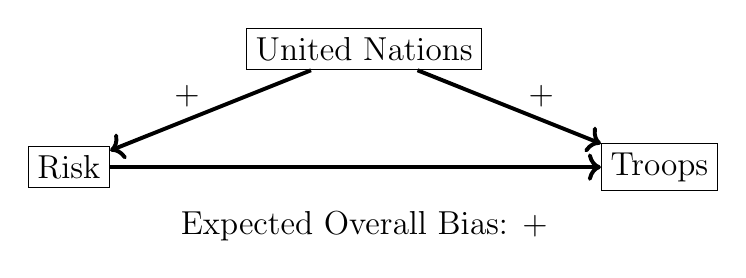
\begin{tikzpicture}[scale=1.5]

% Nodes 
\node[rectangle, draw] at (0, 0) (l) {\large Risk} ; 
\node[rectangle, draw] at (5,0) (r) {\large Troops} ; 
\node[rectangle, draw] at (2.5, 1) (t) {\large United Nations} ; 
\node at (1, 0.6) (s1) {\large $+$} ; 
\node at (4, 0.6) (s2) {\large $+$} ;
\node at (2.5, -0.5) (dir) {\large Expected Overall Bias: $+$} ;

% Lines 
\draw[->, line width = 0.5mm] (l) -- (r) ; 
\draw[->, line width = 0.5mm] (t) -- (l) ; 
\draw[->, line width = 0.5mm] (t) -- (r) ; 


\end{tikzpicture}
\end{center}
\caption{Directed Acyclical Graph of Endogenous Relationship}
\label{fig:Figure 7}
\end{figure}

\begin{singlespace}

Scholars in the peacekeeping literature have noted how relationships involving peacekeepers likely suffer from endogeneity \citep[Ex.][]{fortna2004,fjelde2019}, but these forms of endogeneity bias against their results. I argue that my statistical model likely experiences bias in the same form. To explain the expected endogeneity, I use a Directed Acyclical Graph (DAG)\footnotemark[19] in Figure \ref{fig:Figure 7} to clarify my expectations. The DAG visualizes the relationship between risk, the independent variable, and troops, the dependent variable, that is confounded by an unobserved factor, labeled the United Nations. To estimate an unconfounded causal effect, peacekeeping operations would need to be randomly assigned, but the unobserved factor rooted in the United Nations inhibits random assignment. This unobserved factor can be conceptualized as the United Nation's desire for the the mission to be successful. When the United Nations forms a mission, the Security Council seeks to provide the mission with enough resources to fulfill the mandate and support international peace \citep{allen2014}. These resources include the number of troops contributed by each contributing country. By increasing the count of contributions, the mission will have an increased likelihood of establishing peace \citep{hultman2016united}. As a result, I expect that United Nations' desire for mission success is positively correlated with the contribution of troops. To give the mission its best chance of success and to limit negative externalities of conflict, the United Nations will include tasks relating to reducing battle deaths \citep{hultman2014beyond}, protecting civilians \citep{hultman2013united}, and reducing the duration of conflict \citep{hultman2016united}. This is especially observed with the rise of robust mandates \citep{lloyd_diss}. As a result, the United Nations will add tasks such as Chapter VII enforcement, the protection of civilians, and monitor buffer zones that increase the risk of peacekeeping mandates. This leads me to expect that the United Nations desire for mission success will increase risk. Since both theoretical relationships between the unobserved variable and observed variables exhibit a positive association, I can conclude that my expected bias is positive and biasing in favor of null findings. Had this unobserved characteristic been measured, by results would be more convincing.

In addition to endogeneity concerned with the non-random assignment of a mission, this study rests on a potentially troublesome assumption. The deterrent effect of mandate risk works under the assumption that all mandate tasks require the same number of troops to successfully complete the task. However, in reality, this is likely not the case leading bias that I believe favors of the null hypothesis. The Untied Nations does not provide official recommendations on troop sizes required to complete each task, but rather leaves these decisions up to the preferences of the mission force commander. In a manual on the use of force provided by the Department of Peacekeeping Operations, the United Nations recommends that force commanders consider factors such as military capabilities, force safety, and security of mission personnel when considering the use of force. Force commanders must mitigate risks associated with the conflict environment and the use of force suggesting the possibility of inaction, but force commanders are held accountable for their inaction or failure to protect, especially in situations where lives are at risk \citep{Use_Force}. In the United Nations Infantry Battalion Manual, commanders are instructed to create military units that are equipped to provide self-protection while also deterring potential threats in hostile environments to demonstrate the United Nations' credibility and legitimacy \citep{Infantry}. In the face of risky mission environments, and the potential of being reprimanded for inaction or failure, force commanders prefer to send larger units as a costly signal of deterrence. To effectively send a costly signal of deterrence the mission must be able to use force requiring the associated tasks that increase mission risk. With this in mind, force commanders will prefer to have larger military contingents when dealing with risky tasks biasing towards larger troops contributions. This suggests that my models are a more difficult test of my theoretical argument. 

\end{singlespace}
\end{comment}
\clearpage

\begin{center}
\section{}
\setcounter{table}{0}
\end{center}

\begin{doublespace}
Below, I explain the classification of tasks between ``risky'' and ``less risky'' tasks found in \cite{lloyd2021}. In general, risky tasks are those that make peacekeepers potential targets of conflict, demand the use of force, or are naturally dangerous. 

\vspace{1em}

\subsection*{Monitoring Peace Agreements}

The main task of monitoring a peace agreement and its subtasks of monitoring the buffer zone and liaising war parties are classified as risky tasks while promoting good offices is classified as less risky. Conflicts that end in a peace agreement are more likely to reoccur \citep{fortna2004,walter2009} increasing the likelihood of peacekeeper use of force.

Monitoring a buffer agreement was explained in the main body of the paper, but I will provide a brief summary. This tasks is considered risky since peacekeepers monitor and patrol a combat zone that splits the warring sides that is likely to be the sight of any further conflict. 

Liaising war parties requires the peacekeepers to create effective lines of communication between the warring parties by visiting their respective field headquarters. Peacekeepers vulnerable when entering warring party field headquarters, but this risk is greater when visiting rebel headquarters as rebel groups likely see peacekeeper-government relations as an act of conspiracy against the group. This puts peacekeepers at risk of being a target of conflict \citep{fjelde2016}.

The promotion of good offices, while a subtask of monitoring a peace agreement, is considered less risky. An interview with a former Deputy Special Representative to the Secretary General explains that promoting good offices is another mode to create warring party communication. The mission acts as a mediator to carry messages or create peaceful contact between warring parties without directly taking part in the negotiations \citep{della-giacoma_2015}. As a result, I categorize the promotion of good offices as less risky. 

\subsection*{Peace Agreement Implementation}

The task to implement the peace agreement takes monitoring the peace agreement task on step further making this a risky task. To implement the peace agreement, the mission takes an increasingly active role by enforcing the peace agreement crafted by the warring parties with the use of force. Since peace agreements are less durable compared to decisive military victory \citep{fortna2004,walter2009} and emphasize peacekeeper use of force, I classify this task as risky. 

\subsection*{Monitor Human Rights}

The main task of monitoring human rights and its subtask of monitoring the refugee situation are classified as risky tasks. Missions tasked to monitor human rights require peacekeepers to investigate reports of human rights abuses. Many of these abuses are by-products of conflict such as the killing of civilians \citep{hultman2013united} or sexual exploitation and abuse \citep{johansson2019,kirschner2019}. As a result, missions are likely to move to these dangerous locations to monitor human rights abuses making it a risky task.

I classify monitoring the refugee situation as a risky task. Refugee movements contain rebels hiding in human camouflage, weapons, and individuals with revolutionary ideologies \citep{beardsley2011}, which puts peacekeepers at risk of being targeted or using force. 

\subsection*{Protect Human Rights}

I classify the main task of protecting human rights and the subtasks of protecting children, protecting women, and protecting civilians as risky tasks. The human rights abuses are by-products of conflict \citep{hultman2013united,johansson2019,kirschner2019}. Furthermore, warring parties kill civilians or commit sexual violence improve its relative bargaining position by undermining the opposing side's support base \citep{fjelde2014,fjelde2019,cohen2013}. To deter these human rights violations, especially when protecting children, women, and civilians, peacekeepers move to conflict locations to enforce the protection of human rights. As a result, I consider this main task and its subtasks as risky. 

\subsection*{Protect UN Personnel}

I classify the main task of protecting United Nations personnel as a risky task. Military troops can be called protect United Nations personnel, such as other troop units, United Nations police, and civilian units \citep{Infantry_2012}. Troops are expected to use force to protect United Nations personnel making peacekeepers likely targets. As a result, I classify the protection of UN personnel as a risky task. 

\subsection*{Assist in Demining}

I classify the task of assistance with demining as a risky task. This task requires peacekeepers to remove landmines from the combat zones to protect civilians or other potential victims from danger. These mines may be hidden and remain active long after the conflict subsides. Peacekeepers called to remove mines must exercise high caution to avoid injury or death natural to removing these explosives \citep{demining}. Due to the danger associated with removing mines, I classify this task as risky. 

\subsection*{Refugees Assist}

The main task of assisting the refugee situation is classified as a risky task. Assisting refugees exposes peacekeepers to potentially hazardous situations as refugee groups are host to rebels in human camouflage and arms trafficking \citep{beardsley2011}. Furthermore, assisting refugees forces peacekeepers to facilitate refugee movement across borders, which is a common battle ground for warring parties and border hoping rebels \citep{townsen2014}. As a result, I classify assisting refugees as a risky task. 

\subsection*{Facilitate the Delivery of Humanitarian Assistance}

I classify the main task to facilitate the delivery of humanitarian assistance and its subtask of protecting humanitarian personnel as risky tasks. Humanitarian aid workers are an increasingly vulnerable target, especially in the presence of conflict. Humanitarian aid workers are drawn to protect and help those who may be or are caught in civil conflict or those who do not have necessary resources. Due to the dynamics of conflict, humanitarian aid workers are increasingly killed as a direct or indirect product of conflict \citep{hoelscher2017conflict}. Since peacekeepers are likely to use force to protect humanitarian deliveries and workers, I classify these tasks as risky. 

\subsection*{Monitor Borders}

I classify the main task of monitoring the host state's borders as a risky task, but I classify the subtasks of monitoring the weapons embargo, monitoring the trade of weapons, and the inspection of cargo as less risky tasks. Host state borders are home to the facilitation of refugees and are the site of warring party confrontations that create conflict risk \citep{beardsley2011,townsen2014}. As a result, I classify the task of border monitoring as a risky task.

In contrast, I classify the subtasks of monitoring the weapons embargo and cargo inspections as less risky tasks. Monitoring an arms embargo and the weapons trade requires peacekeepers to deliver information on the flow of arms into the country. In the case of cargo inspections, peacekeepers inspect cargo in safe locations such as ports, airports, and the occasional military base and host state border \citep{TAMM_Codebook}. The lack of specificity in mission mandates on how to carry out these tasks lead to principal-agent problems as peacekeepers shirk their responsibility leading to a lack of engagement with risky environments \citep{bellamy2010}. Second, the majority of shipping locations are less conflict prone since private businesses are risk averse \citep{morrow1998}. As a result of these considerations, I classify these subtasks as less risky. 

\subsection*{Monitor Use of Natural Resources}

I classify the task to monitor the use of natural resources as a less risky task. It is understandable that scholars may think that the monitoring of natural resources should be considered a risky task since many civil conflicts feature conflict over natural resources \citep{lujala2009}. However, peacekeepers are not charged to protect and monitor the resources, but rather to provide advice to governments on how to manage their natural resources \citep{res_2556} making this an advisory action. As a result, I classify this task as a less risky task.

\subsection*{Chapter VII Authorization}

I classify the task of Chapter VII authorization as a risky task. The United Nations Security Council provides Chapter VII authorization to use force in the development and duration of peace. This task allows the mission to take overt military action to combat threats to peace with more force compared to Chapter VI authorized missions \citep{PKO_Ox}. Due to the authorization of the use of overt military action, I classify Chapter VII authorization as risky. 

\subsection*{Elections}

I classify that main tasks of monitoring elections, providing security for the elections, and assisting with election implementation as less risky tasks. Monitoring elections requires peacekeepers to provide technological, logistical, and administrative support to ensure that the election process is smooth. During election assistance, peacekeepers have a more active role by assisting the acting government to organize, monitor, and carry out elections \citep{TAMM_Codebook}. This actions do not demand peacekeepers to use force or engage in conflict making it a less risky task.

Similar to the previous election related tasks, I classify the provision of election security as a less risky task. Peacekeepers charged with electoral security raise the costs of election violence creating a strong deterrent effect on election violence. In addition, elections are normally implemented once the conflict has subsided \citep{fjelde2021protecting}. This allows peacekeepers to avoid the negative externalities of conflict making election security a less risky task. 

\subsection*{Build Government Capacity}

I classify the main task of building government capacity and the subtask of government policy implementation as less risky tasks. Peacekeepers are given the responsibility to re-establish government authority, especially through the use of political and administrative reform. Furthermore, when missions have the responsibility to implement these reforms, the mission will act in an administrative role \citep{TAMM_Codebook}. Due to the peacekeepers acting in an administrative role, I classify these tasks as less risky. 

\subsection*{Preserve Cultural and Historical Sites}

I classify the protection of cultural heritage sites to be a less risky task. This task requests that peacekeepers assist, when necessary and feasible, to protect cultural and historical sites alongside government authorities and the United Nations Educational, Scientific, and Cultural Organization (UNESCO) \citep{TAMM_Codebook}. The task to protect cultural sites has two important qualities that make this task less risky. First, peacekeepers assist the host government and UNESCO instead of being the main enforcers of protection. Second, the task should only be carried out when necessary and feasible suggesting that this is not a high priority task limiting potential danger. As a result, I classify the protection of cultural and historical sites as a less risky task. 

\subsection*{Assist in the Implementation of Quick Impact Projects (QIP)}

I classify the task to assist with Quick Impact Projects (QIPs) as a less risky task. QIPs are initiatives funded by the mission to assist local communities by renovating schools, providing safe access to fresh water, creating solar-powered water systems, and weapons-free zones \citep{QIP}. QIPs develop local communities after the decaying effects of civil conflict allowing the mission to reach out to impacted communities instead of engaging with warring parties. As a result, I classify the tasks of QIP implementation as less risky. 

\subsection*{Assist with Justice Sector Reform}

I classify the task to assist with justice sector reform as a less risky task. The Untied Nations pushes missions with this tasks to develop the justice system, strength criminal justice prosecution, and facilitate rule of law reforms. Many of these factors deal with educating state actors to understand the law, increasing accountability and monitoring to find those who break the law, and ensuring the cost of punishment for breaking the law offset the benefits of breaking the law \citep{blair2021}. Due to the educator and reformer role of the mission, I classify this task as less risky. 

\subsection*{Assist with Security Sector Reform}

I classify the main task of assisting with security sector reform and its subtasks of assisting police reform, monitoring the police, and conducting joint patrols with the police as risky tasks. Government security forces are former actors used attack warring parties and civilians. Peacekeepers must reform former combatants while also investigating and tracking culpable rebels groups \citep{lloyd_diss} making this a risky task. The subtasks of assisting police reform, monitoring the police, and conducting joint patrols with the police follow follow a similar logic. Assisting the police requires peacekeepers to not only impart principles and best practices, but it also requires peacekeepers work with police to create and protect a peaceful environment. Monitoring the police requires peacekeepers to carryout police reform among the police units, but also to ensure the police support human rights further putting peacekeepers at risk. Last, conducting joint patrols with the police requires troops to work alongside the police in the monitoring and patrolling of dangerous locations with high levels of crime, suggesting continued risk to troop physical integrity \citep{TAMM_Codebook}. As a result of potential peacekeeper harm, I classify these subtasks as risky. 

\subsection*{Promote National Reconciliation}

I classify the main task of promoting national reconciliation and its subtask of pursuing justice for war criminals as less risky tasks. The process of national reconciliation is a political action by peacekeepers as mediators to promote trust and reduce social tensions between the warring parties \citep{Pol_Sol}. Due to its political and social nature, I classify this task as less risky. I also classify the subtask of pursuing justice for war criminals as a less risky task. With this task, peacekeepers take an investigative role to search for human rights violators. Instead of looking to combat these individuals, peacekeepers investigate crimes and assist police units in bringing in criminals \citep{TAMM_Codebook}. With this in mind, I classify this subtask as a less risky task. 

\subsection*{Disarmament, Demobilization, and Reintegration (DDR)}

I classify the main tasks of monitoring and assisting with disarmament, demobilization, and reintegration (DDR) as risky tasks. DDR takes weapons that are surrendered by former armed groups and aids their reintegration into society. Peacekeepers must deal directly with armed groups in order to carry out this task putting the troops in a precarious situation \citep{DDR}. Peacekeeping troops are not responsible for the placement of former combatants into job skill programs, but they are more responsible to gather information on the DDR program, guard weapon and ammunition stockpiles from would-be spoilers, providing safe transportation of weapons, and proactively engage with warring parties \citep{Infantry_2012}. As a result of the high potential to engage with frustrated armed combatants and would-be spoilers, I classify the monitoring and assisting with DDR tasks as risky. 

\subsection*{Disseminate Info About the Mission to the Public}

I classify the main task of disseminating info about the mission the public as a less risky task. Peacekeepers act as information sharing agents by sharing with local communities and the warring parties about the role of the mission through radio broadcasts and community outreach \citep{TAMM_Codebook}. Due to the community outreach nature of this task, I classify this task as less risky. 

\subsection*{Promote Freedom of the Press}

I classify the main task to promote press freedom as a less risky task. Peacekeepers have the responsibility to strengthen the legal and regulation frameworks to protect the media and other forms of societal communication while also promoting media professionalization \citep{TAMM_Codebook}. Due to the legal reformation approach of peacekeepers, I classify this task as less risky. 
\end{doublespace}

\pagebreak

\newpage % Page break to seperate the work from the bibliography. 
\singlespacing

\bibliographystyle{apsr_2} % My citation style is APSR

\bibliography{/Users/treywood/Dropbox/Projects/Active_Projects/Mandate_Contribute/Paper/PKO.bib} % This locates my bibliographic information

\end{document}
